\section{Introdução}

\begin{frame}{Relevância e Objetivo}
  \begin{columns}[T]
    \column{0.55\textwidth}
    \small
    \begin{itemize}
      \item Sistemas reator-separador com reciclo são amplamente estudados, da produção de polietileno a reações exotérmicas e endotérmicas acopladas.
      \item O reciclo aumenta a conversão e a seletividade e reduz etapas de purificação, mas intensifica o acoplamento entre variáveis e a não linearidade, o que torna a análise dinâmica mais desafiadora.
    \end{itemize}

    \begin{block}{Objetivo}
      Caracterizar o comportamento dinâmico de um sistema reator-separador acoplado por reciclo por meio de ferramentas clássicas de análise de sistemas lineares.
    \end{block}

    \column{0.45\textwidth}
    \begin{figure}
      \centering
      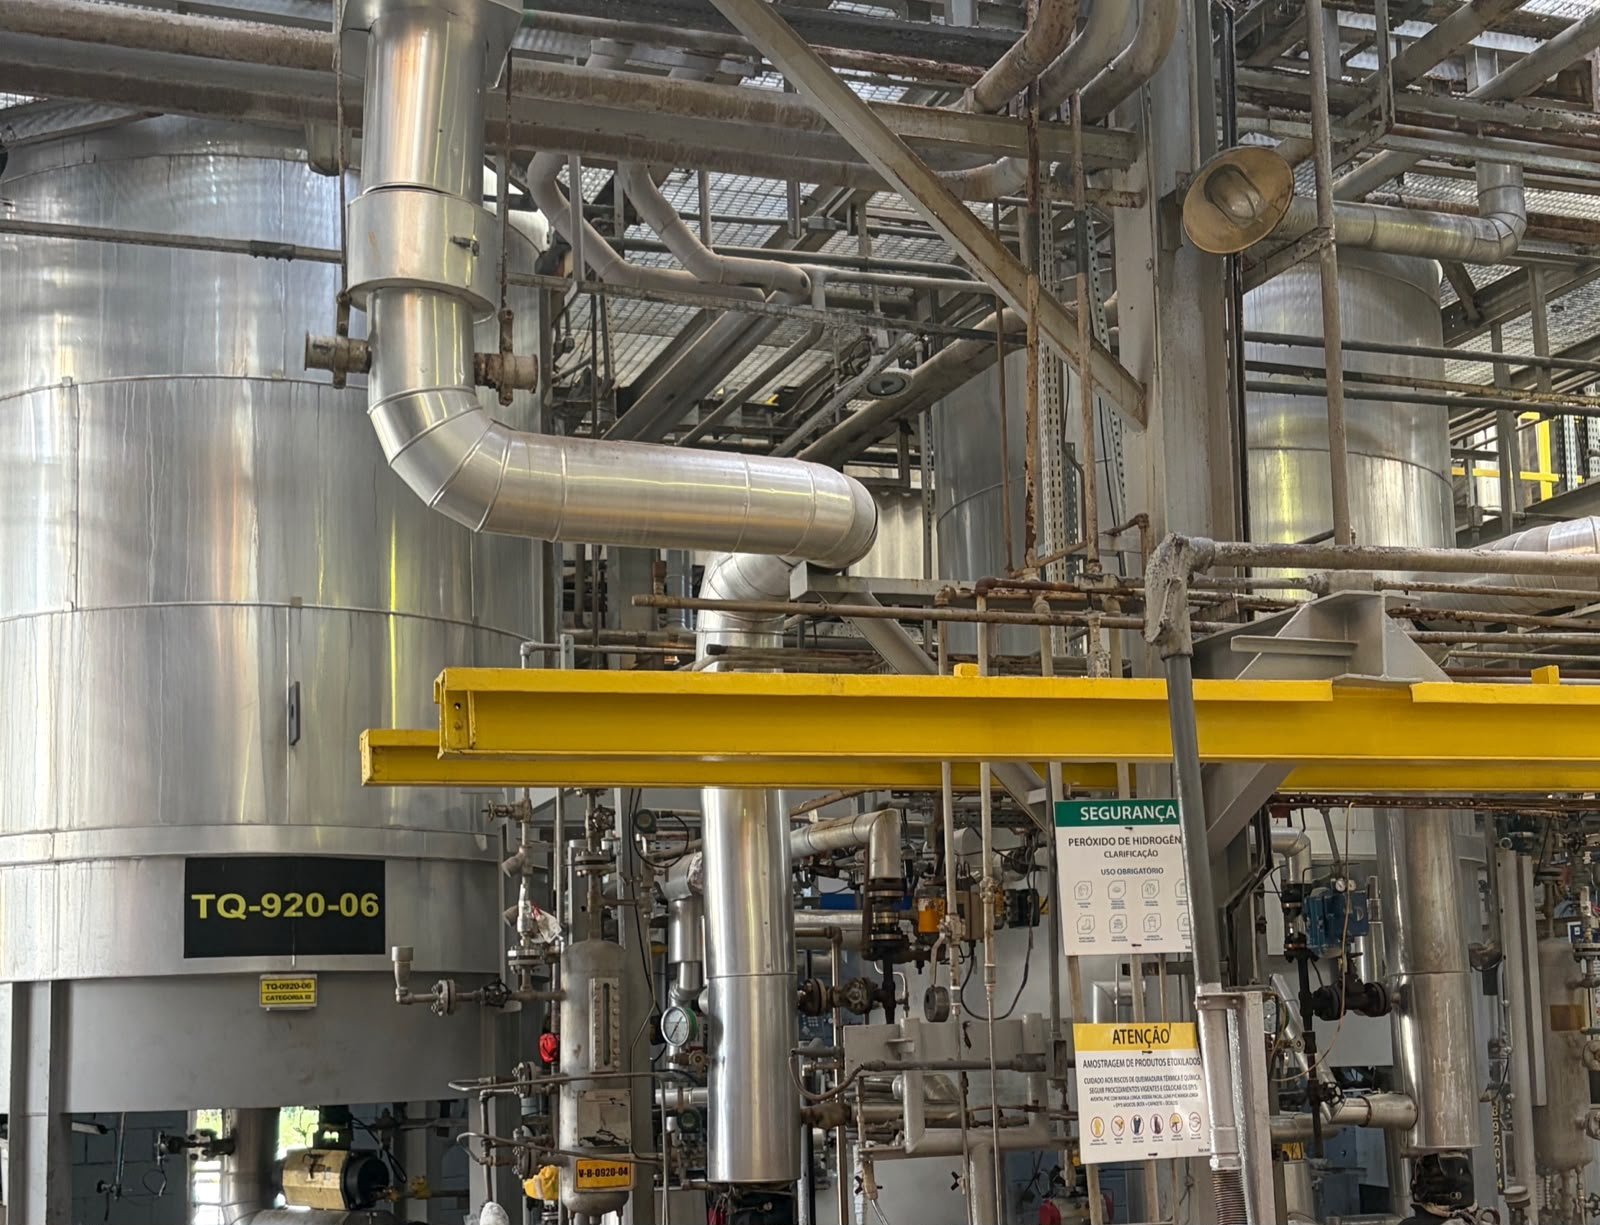
\includegraphics[width=\textwidth]{../figures/indorama.jpg}
      \caption{Unidade de Etoxilação. Fonte: Autores, 2026.}
    \end{figure}
  \end{columns}
\end{frame}
